\title{農業におけるWikiを活用する知の構造化}
\author{プロジェクトマネジメントコース\\
ソフトウェア開発管理グループ\\
矢吹研究室\\
1242034\\
小池 克人}
\date{}
\begin{document}

\maketitle


 \chapter*{謝辞}

\tableofcontents%目次

 \chapter{序論}
\section{title}
\subsection{タイトル}
\subsubsection{小々節見出し}


 \chapter{背景}
平成27年3月10日に発表された農業情報の標準化に関する個別ガイドラインでは,農業の情報の相互運用性を確保するインターオペラビティーとポータビリティー確保の標準化が必要とされている\cite{naikaku2014}.

しかし,異なる企業や団体の意思を一つにまとめる作業には困難が伴う.標準化して,データをやり取りするプロトコルやデータ形式は各企業の利害がぶつかるため,困難である\cite{kizi2015}.よって,複数のシステムの間でマスターを統一しようとする共通語彙には,目的と実現する考え方のアーキテクチャーが異なり,マスターは構造も用語も異なるため現実感が無いため,共通的な方法論ができないかを考える.

作物名称は,研究,行政,流通,農家により変わる.研究は研究目的に応じた分類のため,行政は行政の目的に応じた分類のため,流通は流通に都合の良いネーミングのため,農家は営農の都合に良い分類のための用途により視点が異なる.よって,用語も異なる.

これを目的に応じた用語の変換(翻訳)を実現する共通な仕組みができないかに着目する.用語の変換をするために用語をタグで結び,関連用語を抽出することを考える.これと同じような事例を探し,参考として研究する.そして.2008年のWikipediaの記事構造からの上位下位関係抽出の論文を参考にして,MediaWikiを利用する\cite{nogyo2015}.MediaWikiは,オープンソース(GPL)で配布されているため,MediaWikiを用いれば,自分専用のWikipediaを設置・運用することができる\cite{nico2015}.MediaWikiを利用し,目的に応じて最適な語彙の翻訳を可能とする翻訳システムの開発を研究する.


\chapter{目的}
農業情報の用途により視点,用語が異なる語彙を目的に応じた最適な語彙への翻訳ができるような仕組みを作ることが目的である.

\chapter{農業について}
\section{本章の構成}
本章では,研究対象である農業について解説する.また,農業にに関連する事項も記す.
\section{農業とは}
農業とは,土地を利用して作物の栽培または家畜の飼養を行い,人間にとって有用な生産物を生産する経済活動であり,そのような活動を行う産業である.人間に有用な農業生産物は食糧と一部の工業原料であるが,農業はそれらを,土,水,太陽エネルギーなどの自然力を利用して作物として生産し,また家畜を繁殖,肥育させることによってそれを生産する.このような農業の産業としての特質は,第1に,土地を基本的な生産手段とし,またその土地を商工業などの他産業と比較して,広い面積にわたって相対的に粗放に利用することであり,第2に,人間が長い年月をかけて育成し,または馴らしてきた高等動植物を対象(もしくは手段)とする,有機的生産であることである.\cite{nouwiki2015}
\section{農業の種類}
主な農業の種類を解説する.\cite{kotoba}
\subsection{地中海式農業}
地中海式気候の地域に独特な農業様式のことである.地中海沿岸が代表的で,夏季の高温乾燥に耐えるブドウ,オリーブ,オレンジなどの果樹栽培(おもに丘陵地斜面),冬雨を利用する平地でのコムギ栽培,家畜飼育(ヒツジ,ヤギなど)を組み合わせた農業.
\subsection{酪農}
乳牛を飼育して牛乳および乳製品の生産を行う農業経営.近代的酪農は,早くから有畜の輪栽式農法を行い,畜産物を日常の食品としていたヨーロッパで農業革命後に発展した.
\subsection{園芸農業}
都市への出荷を目的として野菜,果樹,花卉,花木,緑化樹木などを栽培する集約的農業.都市近郊に発達する近郊農業,都市から離れたところに発達する輸送農業などがあり,栽培方法には露地栽培,促成栽培,抑制栽培などがあるが,いずれも都市市場の価格と見合う栽培方法をとっている.
\subsection{混合農業}
種と家畜の飼育を有機的に結びつけた農業.耕種部門では穀物より飼料作物に重点がおかれ,小麦,ライ麦,大麦,じゃがいも,とうもろこしなどを科学的に輪作する.家畜は牛,豚,羊などが多い.
\subsection{プランテーション農業}
熱帯,亜熱帯で行なわれる栽植農業.欧米人が資本,技術を提供し,熱帯の労働に耐え得る先住民や移入労働者の安価な労働力を利用して,モノカルチャー経済を行なう企業的農業経営のこと.作物は貿易品として価値のある香料作物,ゴム,チャ (茶) ,麻,キナノキ,コーヒー,カカオ,サトウキビ,バナナ,タバコなどがある.
\section{品種改良とは}
品種改良とは,生物の遺伝質を人工的に変えて,一段と利用価値の高い新しい型のものを作り出すこと.新しい地域に従来なかった新種,新品種を導入することや,全く新しい生物種を創出することも含む.\cite{kinoko2015}
\section{方法}
主な方法は,別の品種と別の品種を掛け合わせて別の品種を作り,繁殖させる方法が主な方法である.

いろいろな性質のものの中から目的に合ったものを選び出すことで,様々な性質のものが作り出される.

%図の挿入
\begin{figure}[htb]
\centering
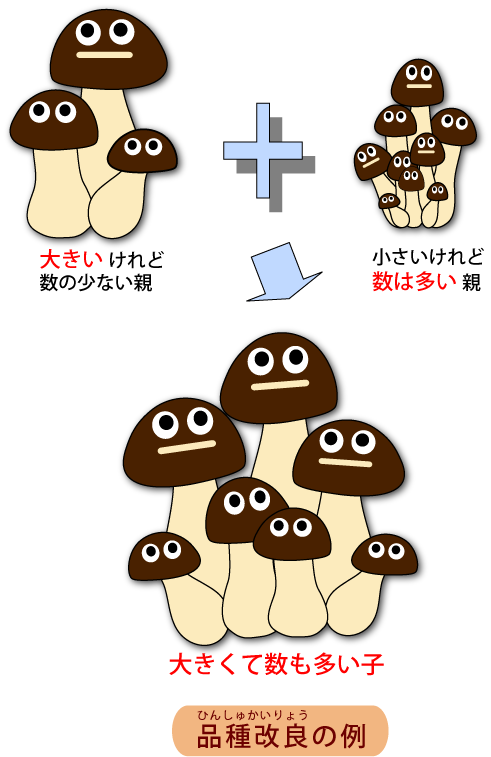
\includegraphics[width=5cm]{kinoko8.png}
\caption{品種改良の例}\label{図}
\end{figure}

\section{遺伝子組み換えとは}
遺伝子組み換えとは,人為的に遺伝子工学の手法を用いて試験管内で遺伝子を組み換えることである.

遺伝子組み換えをGMO,遺伝子組み換えをしない通常のものをnon-GMOと呼ぶ.\cite{kinoko2015}

%図の挿入
\begin{figure}[htb]
\centering
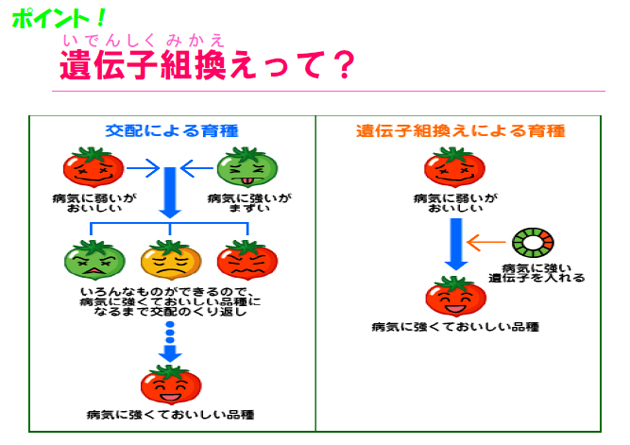
\includegraphics[width=10cm]{iden.jpg}
\caption{遺伝子組み換え}\label{図}
\end{figure}

\subsection{遺伝子組み換えと品種改良の違い}
遺伝子組み換えと品種改良の違いは,人為的か自然に行われるかの違いである.遺伝子組み換えは,人為的に目的の遺伝子を処理するため特定の効果を得るが,品種改良は,自然交配による突然変異種を期待するものである

品種改良は,期待通りのものができるまでに年月がかかる.さらに,確立は,かなり低い\cite{idensi}

\subsection{メリット}
遺伝子組み換えによるメリットは主に,除草剤に耐性と害虫に強くなることが挙げられる.この2つは,栽培するときに農薬をまく回数を減らすため,作業負担を軽減する.そのため,生産へのコストを下げることができる.
\subsection{デメリット}
%図の挿入
\begin{figure}[htb]
\centering
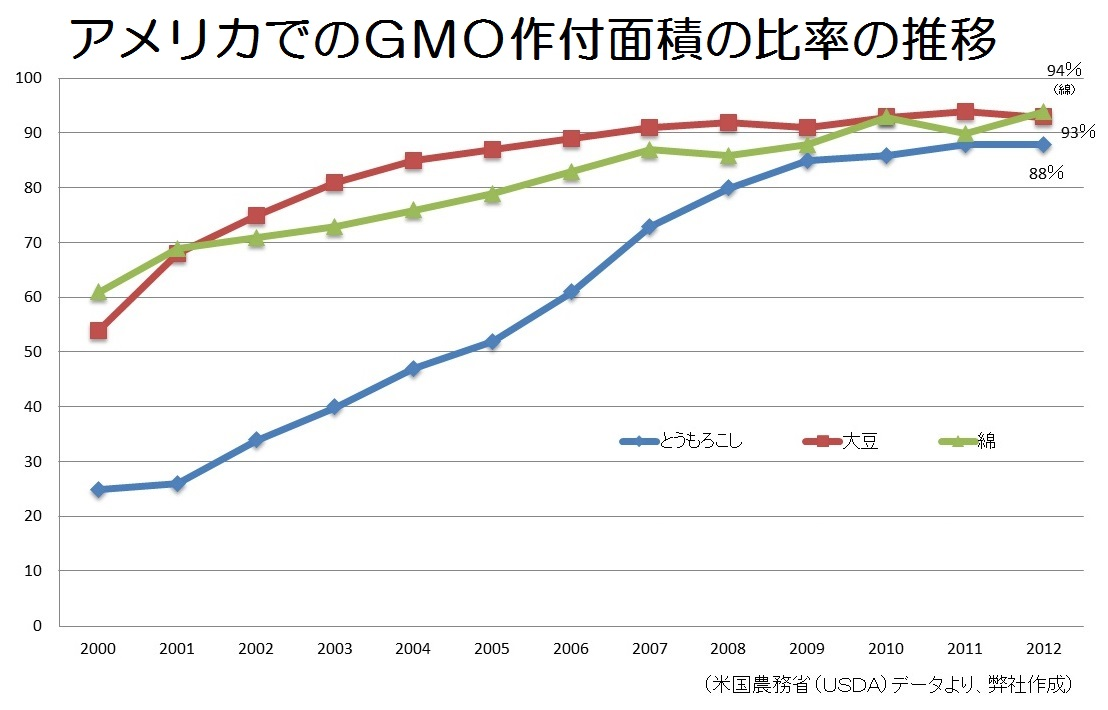
\includegraphics[width=10cm]{GMO.jpg}
\caption{GMO推移比率データ}\label{図}
\end{figure}

デメリットは,健康に健康に悪影響を与える可能性が高いことが挙げられる.アメリカでは,遺伝子組み換えで栽培されているトウモロコシと大豆の比率が高く約9割が遺伝子組み換えになっている.\cite{akikawai}

遺伝子組み換え食品の割合が多いアメリカでは,遺伝子組み換え食品の出現と共にガン,白血病,アレルギー,自閉症などの慢性疾患が急増しているというデータが出ている.このデータが遺伝子組み換えの有害性を断言できるわけではないが,可能性を指摘できる.\cite{mondsi}
%図の挿入
\begin{figure}[htb]
\centering
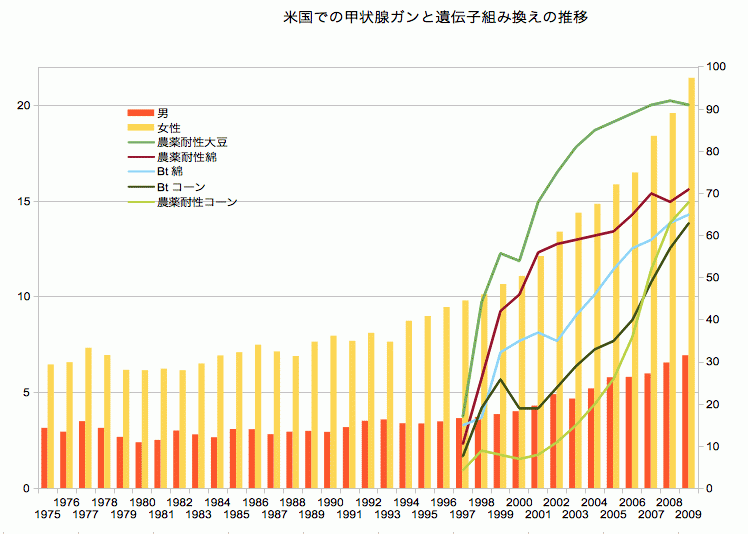
\includegraphics[width=10cm]{gan.png}
\caption{アメリカでの甲状腺ガンと遺伝子組み換えの推移}\label{図}
\end{figure}


\section{現在の農業情報}
現在の農業では,品種改良,遺伝子組み換えをした農作物が大量に存在する.苺で例えると,アイベリー,あかねっ娘,あきひめ,あまおう,あすかルビー,あまおとめ,あわゆき,えちごひめ,エラン,おおきみ,おいCべりーおとめごころ,かおりのと同じ苺でも大量に存在する.

 さらに農作物は,農家,流通,研究,行政によって名称が変わりる.農家は営農に都合の良いように,流通は都合の良いように産地名やブランド名などのために,研究は研究目的に応じた新品種開発や防疫,防虫のために,行政は行政の目的に応じた統計作りや分類のためによって用語や用途が変わる.

\chapter{Wikiについて}
\section{本章の構成}
本章では,研究の対象であるWikiについて基本知識と関連する 解説を記述する .
\section{Wikiとは}
Wikiとは,Webブラウザから簡単にWebページの発行・編集などを行えうことができる,Webコンテンツマネジメントシステム(CMS)の1つである.

複数人が共同でWebサイトを構築していく利用法を想定しており,閲覧者が簡単にページを修正や新しいページを追加することができるようになっている.編集者をパスワードなどで制限,編集できないよう凍結することもできる.HTMLの知識がなくてもリストやリンクを簡単に作成できるようになっており,簡易な整形書式が定められている.

Wikiは,内容の編集・削除が自由なこと,基本的に時系列での整理を行わないことから,誰もが自由に「記事」を書き加えていくコラボレーションツールに近い.柔軟性が高く,手軽に始められて操作が簡単なことから,特定のテーマのまとめサイトの制作に利用されることが多い.\cite{wiki}
\section{特徴}
主なWikiの特徴は3つ挙げられる.\cite{wiki3}
\begin{enumerate}
\item Web上であれば,場所や日時関係なく誰にでも文章を書き換えることができる.
\item 文章を書き換えるのにウェブブラウザのみでできる.
\item HTMLより簡単なマークアップ構文で書くことができる.
\end{enumerate}
\section{歴史}
Wikiのソフトウェアは,デザインパターンの共同体でパターン言語を書くために創られたものである.1995年にウォード・カニンガムが確立したPortland Pattern Repositoryが初のWikiだった.

カニンガムは,Wikiの概念を発明し名付け,Wikiエンジンの初の実装を製作した.元々のWikiだけが,Wikiあるいはウィキウィキウェブと呼ばれるべきだと主張する人もいる.カニンガムのウィキ (Wards Wiki) はいまだに最も人気のあるウィキサイトの1つである.

20世紀の最後の数年に,WIkiは非公開・公開のナレッジベース(知識の基地)を開発するのに有望な技術であるということが,ますます認知されるようになった.そしてこの潜在能力は, Nupedia という百科事典プロジェクトの開祖ジンボ・ウェールズ(Jimmy Donal "Jimbo" Wales)とラリー・サンガー(Lawrence Mark "Larry" Sanger)に,ウィキ技術を電子百科事典の基礎に使おうというひらめきを与えた.

このことからウィキペディアは,2001年の1月に始まった.初めはUseModソフトウェアを基にしていたが,後にいくつかの他のウィキから取り込まれた独自のオープンソースのコード基盤に切り替えられた.

今日においては,一番項目の多いWikiは英語版ウィキペディアといわれる.非英語のウィキペディアも世界でも比較的に大きい.しかし,2004年において世界で二番目に大きいウィキはUseModというソフトを使うスウェーデン語のSusning.nuであったように,ウィキペディア以外のウィキでも大きなウィキは存在する.\cite{wiki}
\section{活用例}
Wikiは,誰でも,ネットワーク上のどこからでも,文書の書き換えができるようになっているため,不特定多数の共同記事を作成することに向いている.

例えば技術ドキュメントや仕様書の作成,会議の議題や議事録の共有,開発部門やサポート部門の間でのナレッジ共有,事例や凡例の共有などの利用方法などが挙げられる.\cite{wikiwiki}

%図の挿入
\begin{figure}[htb]
\centering
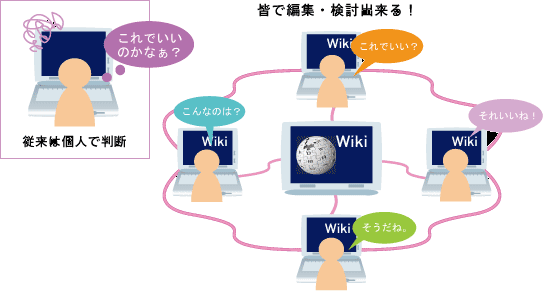
\includegraphics[width=10cm]{img_wiki03.png}
\caption{ウィキの活用例}\label{図}
\end{figure}




\chapter{Wikipediaについて}
\section{本章の構成}
本章では,Wikipediaについて記す.
\section{Wikipedia とは}
Wikipediaとは,2000年に立ち上げられた百科事典Wikimedia Foundation, Incが運営しているインターネット上の百科事典である.Wikipediaは,インターネット上のウェブサイトにアクセス可能な全ての人が自由に編集に参加できる.

使用言語は,288言語あり,世界各国の言語で記事を展開している.日本語の記事だけでも約980,000もあり,全ての記事の数は,約34,000,000記事がある.\cite{wikipedia}

%図の挿入
\begin{figure}[htb]
\centering
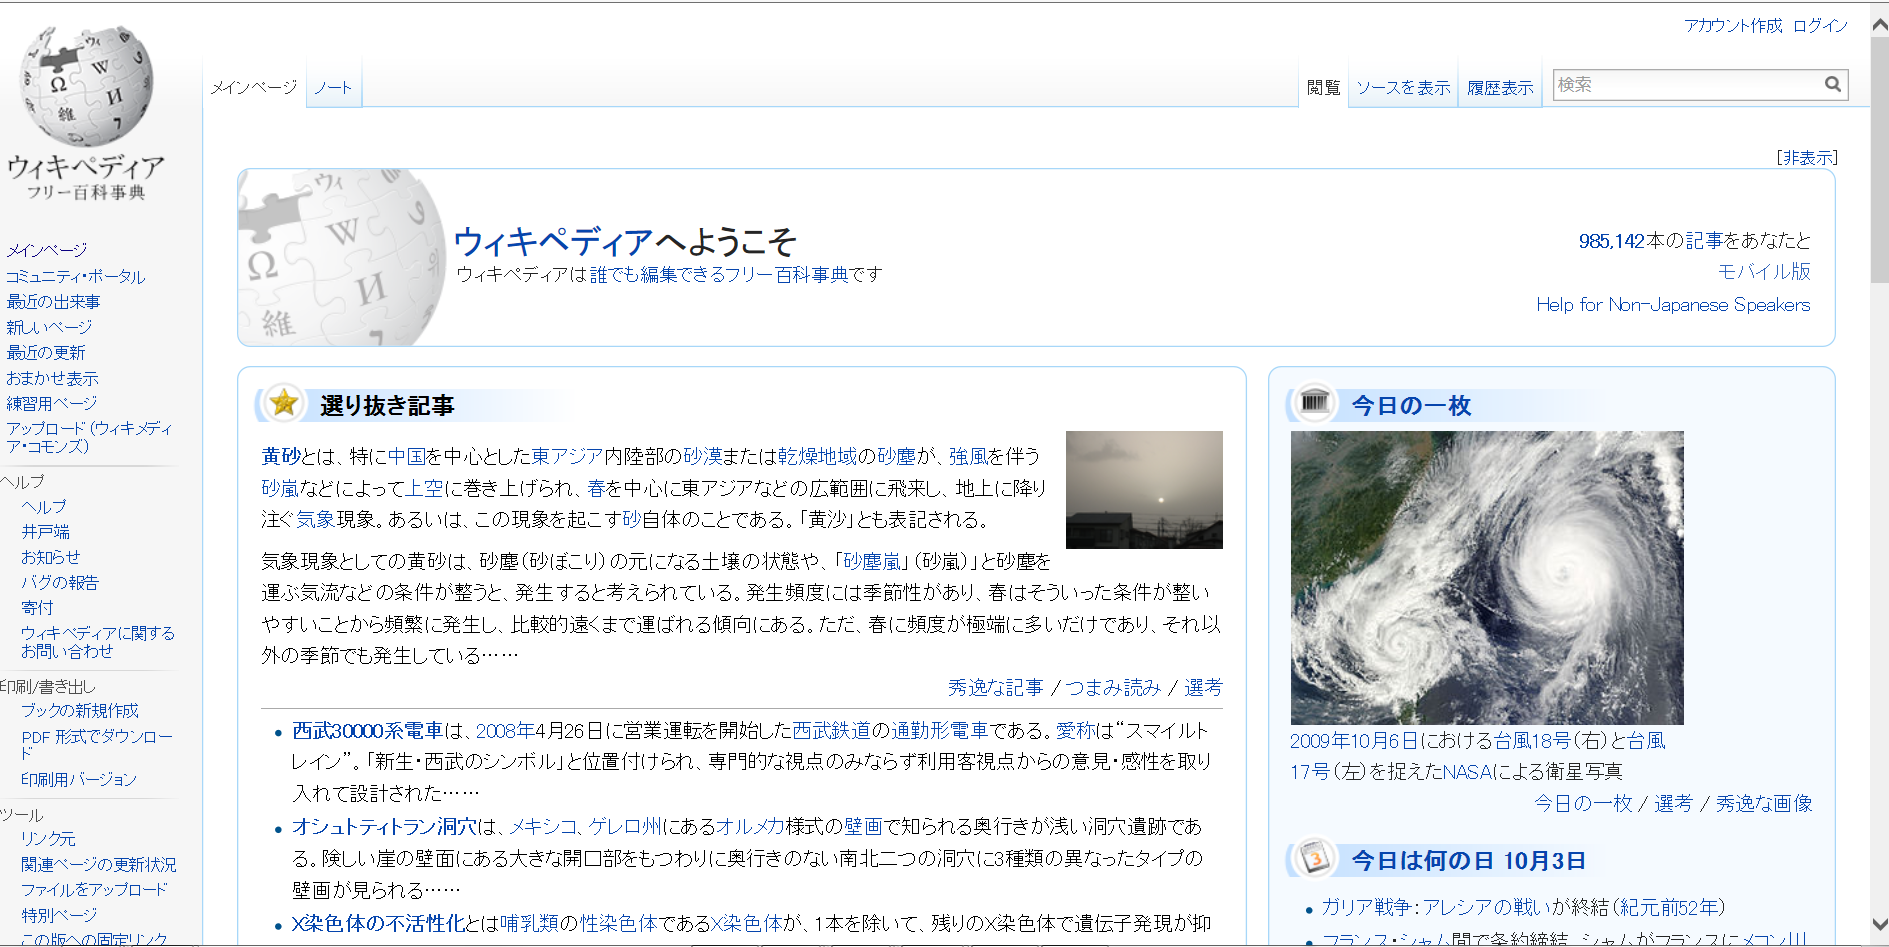
\includegraphics[width=12cm]{wikipedia.png}
\caption{wikipediaトップ画面}\label{図}
\end{figure}

\section{用語}
Wikipediaで主に使われている用語を解説する\cite{yougo}
\subsection{インターウィキリンク}
ウィキ間リンク,Interwikiとも.あらかじめ登録されている他のサイトへ簡便にリンクする方法.ウィキペディア内では,多言語版や姉妹プロジェクトへのリンクを張るのに使われる事が多く,その際に要約に「インターウィキ」 “interwiki“ などと記述される事が多い.
\subsection{ウィキ化}
既存の記事に対して,リンクなどのマークアップを行い,ウィキペディアの一般的なスタイルに整える作業.ウィキファイとも.初稿が文章のみの記述の場合に行われる事が多く,その際,要約欄には「wikify」や「ウィキ化」などと記述される場合が多い.

\subsection{ウィキプロジェクト}
特定の分野について統一的なフォーマットを用意し,ウィキペディア内でのスタイルの統一をはかる場.その分野の記事全体に関わる問題について,広く意見を求めるためにも利用される.
\subsection{ウィキポータル}
特定の分野の記事群に対して入り口となるポータルサイトを用意し,索引,更新情報,新規項目の依頼などその分野に関する情報を提供する場.
\subsection{管理者}
一般の利用者には制限されているいくつかの機能を行使でき,編集合戦や荒らしへの対策としてページを保護や問題のある利用者の投稿ブロックなどを行うことができる.ウィキペディアにおける発言の重みは一般利用者と同じものとされ,一般的に管理者という言葉がイメージさせるような大きな権限はない.
\subsection{サンドボックス}
試し書きや練習用として編集を実際に行なえるページ.一定時間が経つと,投稿した内容は消されるようになっている.ここ以外にも,編集の際に,プレビュー機能を使えばある程度だが代用できる.
\subsection{名前空間}
 端的に言えばウィキペディアの記事が属する分野のこと.ウィキペディアにおける記事名のうち,半角コロン (:) に先行する部分が名前空間名である.ウィキペディアには百科事典としての記事が置かれる通常名前空間やウィキペディア自身についての情報に関する記事が属するWikipedia名前空間のほかにも,利用者名前空間,Template名前空間などいくつかの名前空間がある.
\subsection{ボット}
ロボット(機械)の略語.自動的にウィキペディアの編集を行うプログラム.日本語版では,interlangの体裁を整えるボット,定型メッセージの形式を更新するボットなどが活動している.

\section{編集方法}

ウィキペディアの編集方法は,一部の保護されているページを除いて、全てのページには「編集」と書かれたリンクがありこのリンクをクリックする.


次に,クリックするとそのページのソースの書かれたページが開き,そのページに記述する.

記入し終わったら,編集内容の要約を記入し,「以上の記述を完全に理解し同意した上で投稿する」ボタンを押して保存する.
%図の挿入
\begin{figure}[htb]
\centering
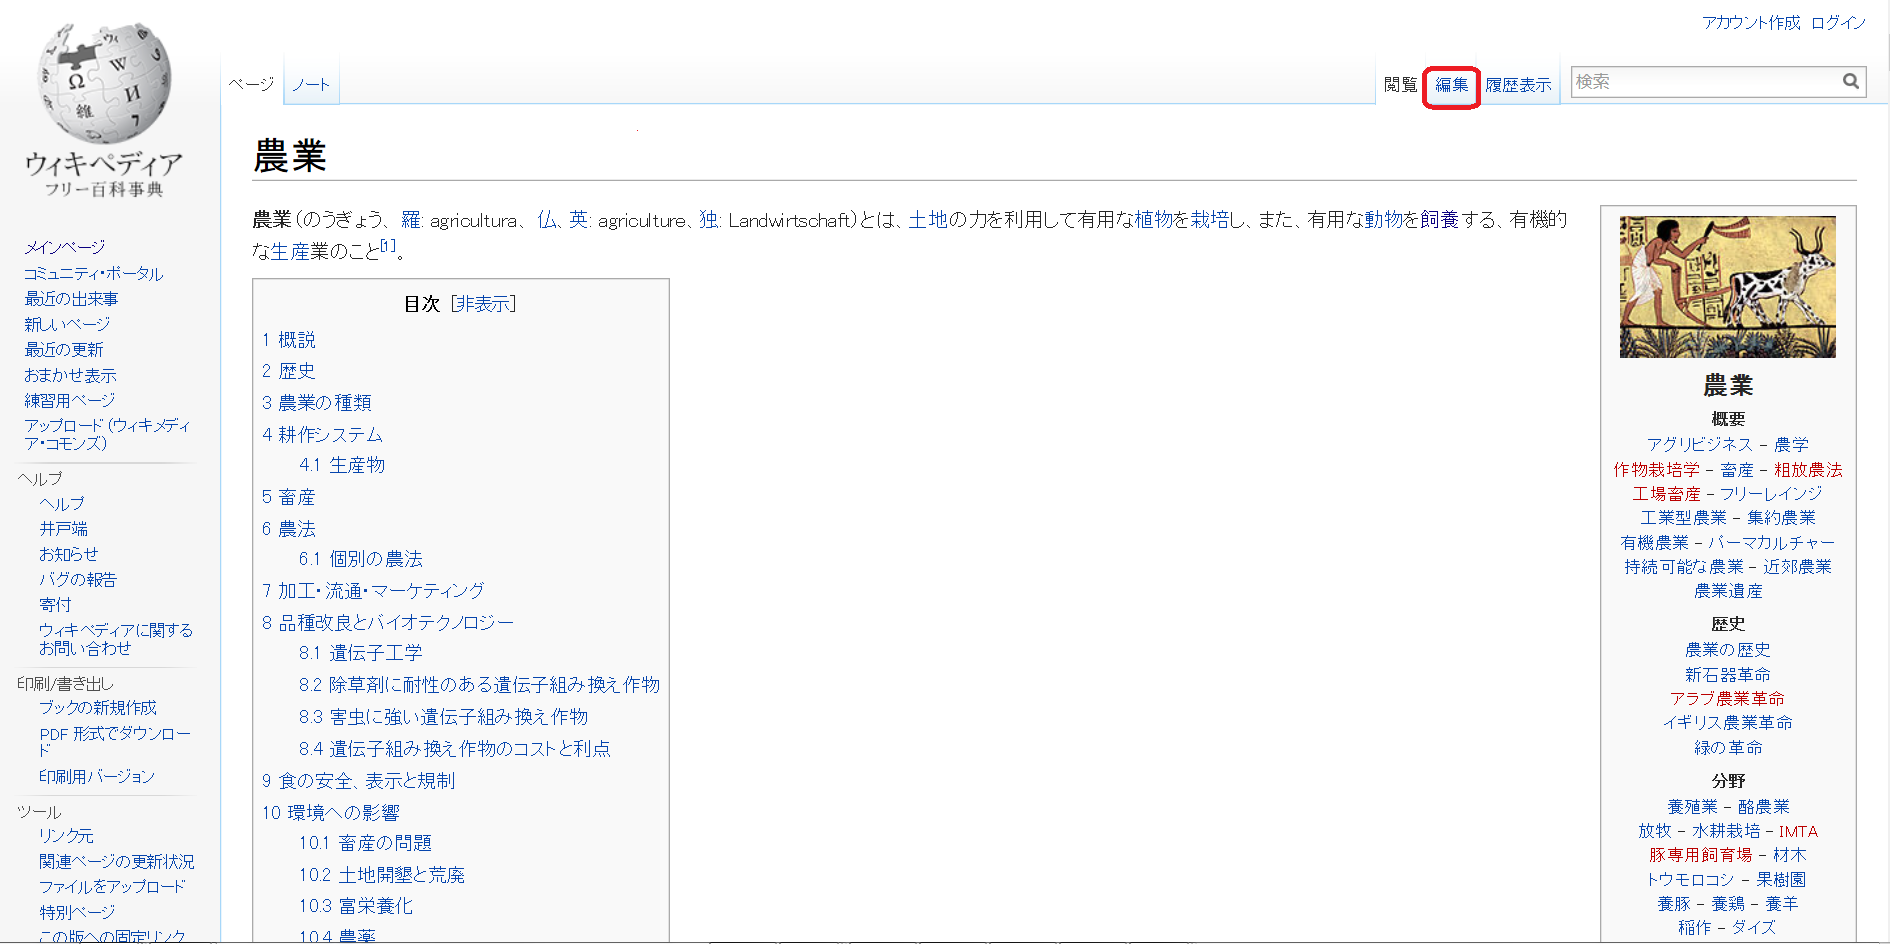
\includegraphics[width=12cm]{mudai.png}
\caption{編集画面1}\label{図}
\end{figure}

%図の挿入
\begin{figure}[htb]
\centering
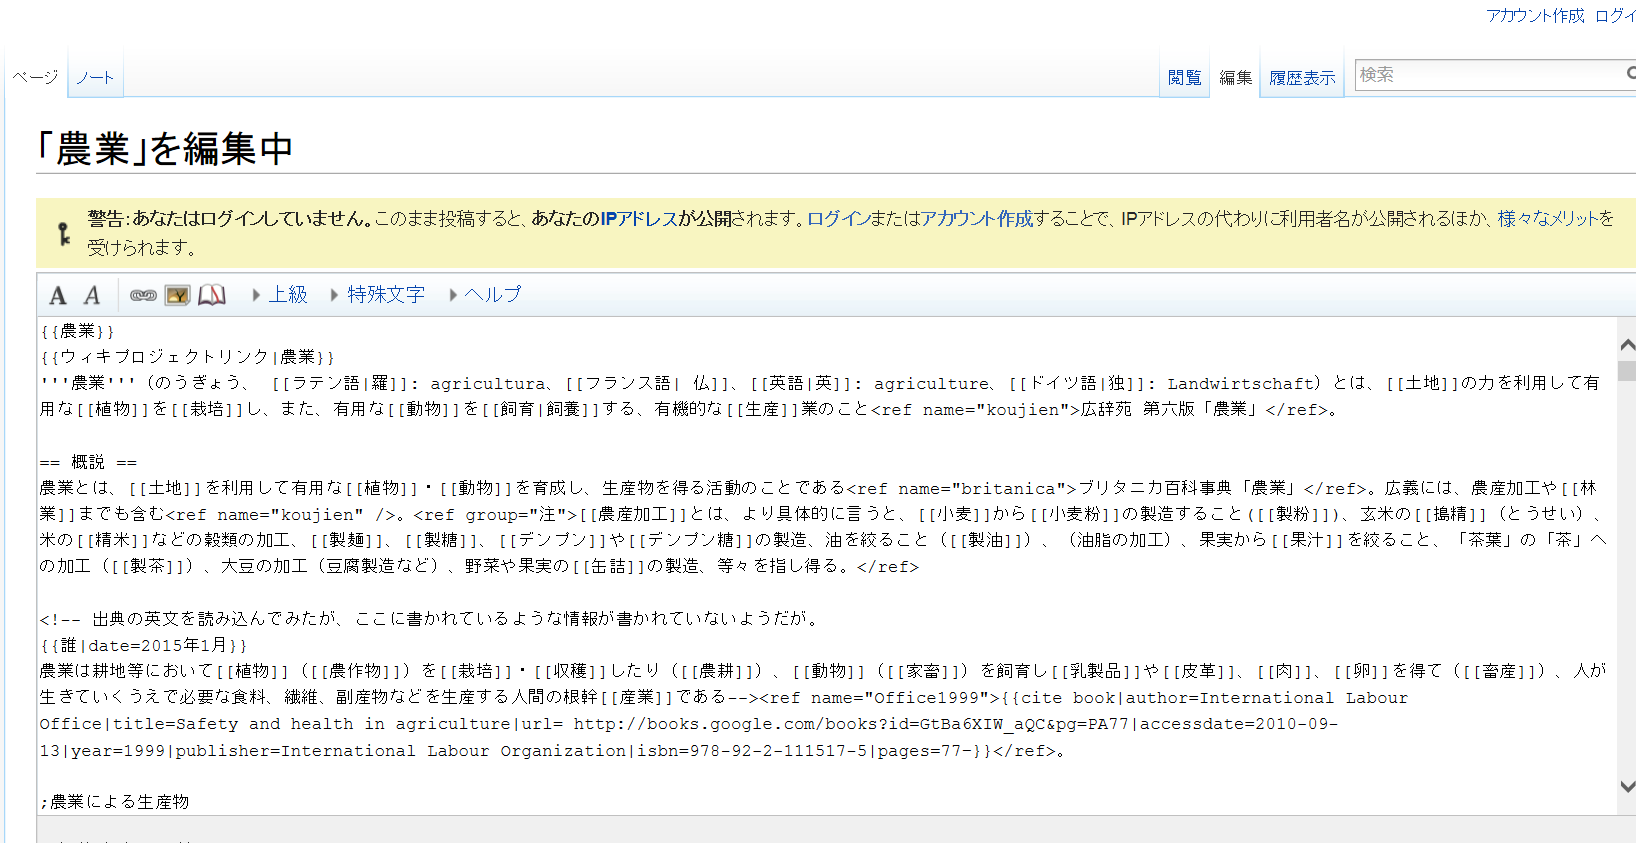
\includegraphics[width=12cm]{2.png}
\caption{編集画面2}\label{図}
\end{figure}

%図の挿入
\begin{figure}[htb]
\centering
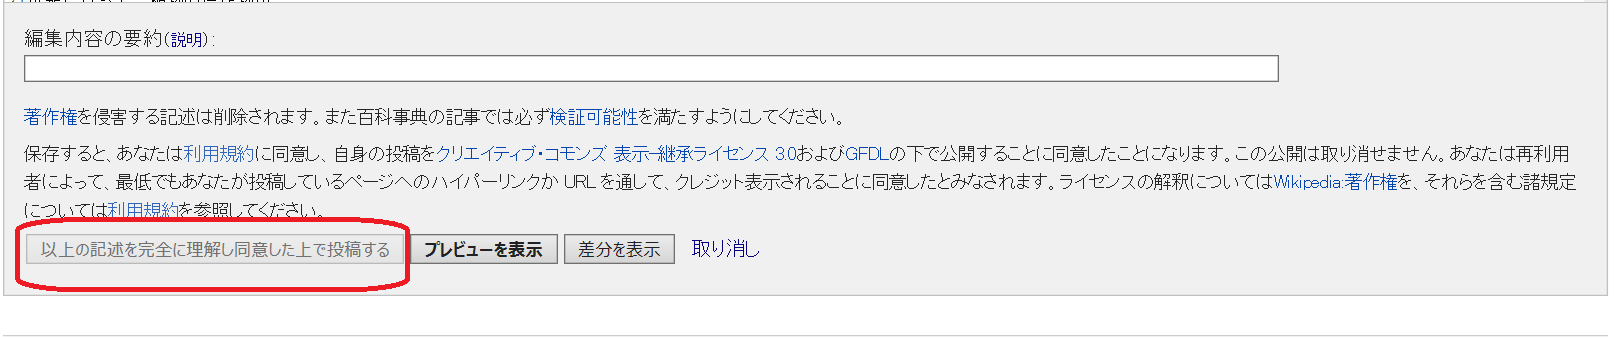
\includegraphics[width=12cm]{3.png}
\caption{編集画面3}\label{図}
\end{figure}

以上が編集の方法である.\cite{rendyuu}

\chapter{Mediawikiについて}
\section{本章の構成}
本章では,本研究で使用するMediawikiの基礎知識について記述する.
\section{Mediawikiとは}
Mediawikiとは,GNU General Public Licenseで配布されるウィキソフトウェアである.PHPで書かれており,データベースとしてMySQLまたはPostgreSQLを使用する.MediaWikiはWikipediaのために作られたシステムで,Wikipediaを運営している.
ウィキメディア財団によって開発されているウィキペディアの為にMagnus Manskeらによって作成された.最初はUseModWikiを使用していたが,2002年1月25日に新しいバージョンに切替えられた. \cite{media}




\chapter{手法}
\section{title}
\subsection{タイトル}
\subsubsection{小々節見出し}


\chapter{結果}
\section{title}
\subsection[タイトル]
\subsubsection{小々節見出し}


\chapter{考察}
\section{title}
\subsection[タイトル]
\subsubsection{小々節見出し}


\chapter{結論}
\section{title}
\subsection[タイトル]
\subsubsection{小々節見出し}




参考文献は文献ファイル(この文書では\verb|biblio.bib|)に記述し,\verb|\cite|で参照する.例:データベースのための	問い合わせ言語SQLで数独を解く方法が提案されている\cite{yabuki2011}.このように参照すると,参考文献リストに自動的に登録される.文献の種類には,雑誌論文\cite{yabuki2011}や会議録論文\cite{yabuki2013},卒業論文\cite{kubo2014},書籍\cite{okumura2013},ウェブサイト\cite{self}などがある.文献の種類によって必要な項目が異なるため,\verb|biblio.bib|を見て確認すること.

\bibliographystyle{junsrt}
\bibliography{biblio}%「biblio.bib」というファイルが必要.

\end{document}
